%%%%%%%%%%%%%%%%%%%%
%%%%% Preamble %%%%%
%%%%%%%%%%%%%%%%%%%%

%This is a simple template for the LaTeX 'article' class document
\documentclass[]{article}%

%These are general packages that we will use quite a bit
%Once you begin using Latex more and more, you will learn what packages suit your needs the best and you can just copy and paste them into any new documents your are creating
\usepackage{amsmath}					%Standard math package built by the American Mathematical Society
\usepackage{amsfonts}					%Standard font package
\usepackage{amssymb}					%Extended symbol collection
\usepackage{amsthm}						%To use the AMS theorem collection
\usepackage{graphicx}					%For when you want to include images or figures into your document
\usepackage{url} 						%For when you want to include a url into your document
\usepackage[hidelinks]{hyperref} 		%For hyperlinking references (NOTE: can remove the [hidelinks] to show link boxes around hyperlinks
\usepackage[usenames,dvipsnames]{color} %This allows me to change the color of my font 
\usepackage{comment}					%For block comments under figures and tables
\usepackage{fancyhdr}					%Allows for a fancy header and footer on your document
\usepackage{lastpage}					%Keeps count of what page number is the last page to be used in the footer
\usepackage{titling}					%Allows for image on title page
\usepackage{hologo}						%Allows for typsetting of the bibtex logo

%Set the margins of the paper using the geometry package
\usepackage[margin = 2cm]{geometry} %This creates a 2 cm margin around the page (NOTE: this does not include the header or footer in the 2 cm cutoff.  If you wanted to you could 										say \usepackage[margin = 2cm, includefoot, includehead]{geometry} which would make it so the header and footer start 2 cm down the page and 										the contents would follow appropriately)


%The following allows for the necessary documents to build the pdf to be embedded into the final pdf file.
%This allows for ease of sharing and automatically generates a back up in a sense in case you lose your .tex file.
%This isn't critical to include but it is nice to know about.
\usepackage{embedfile} 					%Allows embedding of files into the pdf document
\embedfile{MasterGuide.tex} 			%Embed the .tex file into the pdf
\embedfile{MyBib.bib}					%Embed the .bib file into the pdf
\embedfile{./Figs/cat.jpg}				%Embed the .jpg file into the pdf

%This is the standard setup for creating new commands
%The following commands are two that have been regularly throughout this document
%If you want to rename an already defined command, you must use \renewcommand instead
\newcommand{\del}{\partial} 
\newcommand{\bs}{\textbackslash}
\newcommand{\TT}[1]{\texttt{#1}}
\newcommand{\tpc}{\textperiodcentered}

\definecolor{darkgrey}{gray}{0.3}
\newcommand{\greytext}[1]{{\textcolor{darkgrey}{#1}}}

\theoremstyle{definition}
\newtheorem{dfn}{Definition}

%Create the header for the paper
\pagestyle{fancy}				%Makes header in the style of 'fancy', look up LaTeX's fancyhdr to see how you can customize
\lhead{\today}			%Left head
\rhead{MEGC \LaTeX\ Workshop}	%Right head
\cfoot{Page \thepage\ of \pageref{LastPage}}

%%%%%%%%%%%%%%%%%%%%%%%%%%%%%%%%%%%%%%%%%
%%%%% Preamble Ends, Content Begins %%%%%
%%%%%%%%%%%%%%%%%%%%%%%%%%%%%%%%%%%%%%%%%

%Includes figure on title page but needs the titling package to work
\pretitle{
	\begin{center}
		\LARGE
		
\includegraphics[width=0.5\textwidth]{./Figs/MEGC_logo.png}\\[\bigskipamount]
	}
	\posttitle{\end{center}}

\begin{document}
	
	
	%%%%%%%%%%%%%%%%%
	%%%%% Title %%%%%
	%%%%%%%%%%%%%%%%%
	
	%The commands below define and make the titlepage
	\title{Learning \LaTeX\ with MEGC}
	\author{\vspace{1 in} \\University of Michigan 
		\\Ann Arbor, Michigan \vspace{.25 in} \\by: \\Jeff Koller \vspace{1 in}
	} 
	\date{October 1\textsuperscript{rd}, 2015}
	\maketitle				%Create title
	\thispagestyle{empty} 	%Remove header and footer.
	\clearpage				%Equivalent to a page break
	
	
	%%%%%%%%%%%%%%%%%%%%%%%%
	%%%%% Introduction %%%%%
	%%%%%%%%%%%%%%%%%%%%%%%%
	
	\section{Introduction}
	
	\subsection{Editors}
	There are many different \LaTeX\ editors out there.
	This website gives a good overview of the different editors, their benefits and disadvantages, and what operating systems they work on:
	\begin{center}
		\url{http://en.wikipedia.org/wiki/Comparison_of_TeX_editors}.
	\end{center}
	It is important to note that you can do all of your \LaTeX\ using online editors like ShareLaTeX, but you need an internet connection to do so.
	If you wish to work on your local machine (which is typically faster to compile than going through a cloud service) you may want to consider downloading an editor.
	When you download, you will receive a default editor called TeXworks.
	This is a bare bones editor and you could greatly benefit from an alternative.
	Some editors that MEGC members have used or have considered are the following:
	\begin{itemize}
		\item \textbf{Windows:} \url{https://www.youtube.com/watch?v=g6ez7sbaiWc}
		\begin{itemize}
			\item \href{http://www.texstudio.org/}{TeXstudio} $\leftarrow$ \emph{This is T.J.'s favorite editor}
			\item \href{http://www.xm1math.net/texmaker/}{Texmaker} $\leftarrow$ \emph{This is Jeff's favorite editor}
			\item \href{http://www.texniccenter.org/}{TeXnicCenter} $\leftarrow$ \emph{This editor is not our favorite, but is the most widely used on Windows OS}
		\end{itemize}
		\item \textbf{Mac OS:} \url{https://www.youtube.com/watch?v=5CNmIaRxS20}
		\begin{itemize}
			\item \href{http://pages.uoregon.edu/koch/texshop/}{TeXShop} $\leftarrow$ \emph{Sara's go to editor on Mac}
			\item \href{http://tacosw.com/latexian/download.php}{Latexian} $\leftarrow$ \emph{Does live previewing but somewhat out of date}
		\end{itemize}
		\item \textbf{Ubuntu (Linux):} \url{https://www.youtube.com/watch?v=g6ez7sbaiWc}
		\begin{itemize}
			\item \href{https://apps.ubuntu.com/cat/applications/texmaker/}{Texmaker}
			\item \href{https://apps.ubuntu.com/cat/applications/precise/gummi/}{Gummi} $\leftarrow$ \emph{Brandon's go to editor in Ubuntu and has live previewing}
			\item \href{https://apps.ubuntu.com/cat/applications/kile/}{Kile} $\leftarrow$ \emph{Sara's go to editor in Ubuntu}
			\item \href{https://www.gnu.org/software/auctex/}{AUCTeX} $\leftarrow$ \emph{Works with Emacs}
		\end{itemize}
	\end{itemize}
	
	\subsection{Syntax}
	\begin{itemize}
		\item Command Syntax
		\begin{itemize}
			\item For the most part, every command in \LaTeX\ can be described as \TT{\bs command[options]\{argument\}}.
		\end{itemize}
		%
		\item Environments
		\begin{itemize}
			\item Writing in \LaTeX\ can be thought of as writing in multiple different environments.
			You can have text environments, math environments, table environments, figure environments, and many many more.
			These environments can be nested and are typically marked by \TT{\bs begin\{\tpc\}} and \TT{\bs end\{\tpc\}} where what is inside of \TT{\{\tpc\}} denotes the environment.
			By default you are usually in the text environment when writing a document.
			%
			\item One exception to the \TT{\bs begin\{\tpc\}} and \TT{\bs end\{\tpc\}} markings is when you switch between text and math environments while keeping the math inline with the text.
			This switch is marked by \TT{\$\tpc\$}, but we will get to more of this in Section \ref{sec:math}.
		\end{itemize}
	\end{itemize}
	
	\subsection{Components to a \LaTeX\ Document}
	\begin{itemize}
		\item Preamble
		\begin{itemize}
			\item The preamble sets up the document by telling \LaTeX\ what document type you are working on, what the page layout should look like, what packages you plan to use, and allows you to define new commands.
			The preamble is everything before the \TT{\bs begin\{document\}} command.
		\end{itemize}
		\item Content
		\begin{itemize}
			\item The content of the \LaTeX\ document is everything between the \TT{\bs begin\{document\}} command and the \TT{\bs end\{document\}} command.
			This includes everything that you see in the finalized PDF document.
			By default the \TT{document} environment is a text environment.
			Everything you write between \TT{\bs begin\{document\}} and \TT{\bs end\{document\}} will be plain text unless an alternative environment is indicated.
		\end{itemize}
	\end{itemize}
	
	\subsection{Document Class}
	There are many different classes of documents you can write in \LaTeX.
	The document class can be thought of the style that you are writing in.
	The document class is defined at the top of the preamble (line 6 in this .tex file) and is generally denoted by \TT{\bs documentclass[options]\{class\}}.
	\begin{itemize}
		\item \TT{article} - for short documents such as a publication (this document)
		\item \TT{report} - for longer technical documents; like articles, but has chapters 
		\item \TT{book} - for large documents, such as books 
		\item \TT{letter} - for writing letters (has other special properties which have to be set) 
	\end{itemize}
	A full list of document classes and class options can be found here: \url{https://en.wikibooks.org/wiki/LaTeX/Document_Structure#Document_classes}.
	
	\subsection{Packages}
	Packages are essentially libraries of commands that you are telling \LaTeX\ you will be using throughout the document.
	Packages may be needed for specific mathematical symbols, fonts, colors, the ability to insert figures, the ability to change document formatting, and much much more.
	An example of a package used in this document is the following:\\
	\begin{center}
		{\TT{\bs usepackage[margin = 2cm]\{geometry\}}}
	\end{center}
	The package \TT{geometry} allows for an easy way to customize the document margins.
	The option \TT{[margin = 2cm]} allows for a 2 centimeter margin all the way around the page without including the header or footer in that cutoff (ie the header and footer are within 2 centimeters of the paper's edge).
	We could change the option to \TT{[margin = 2cm, includefoot, includehead]} to make sure that the header and footer are outside of this margin cutoff as well.
	The option \TT{margin} can also be changed to \TT{top}, \TT{bottom}, \TT{left}, and \TT{right}.
	You can always look up a package name to figure out the specific options for that given package.
	Take a minute to try changing the options on the \TT{geometry} package in the preamble to see how it effects this document.
	%
	\clearpage
	
	%%%%%%%%%%%%%%%%%%%
	%%%%% Writing %%%%%
	%%%%%%%%%%%%%%%%%%%
	
	\section{General Writing with \LaTeX}
	In this section, we are mainly going to talk about general writing in \LaTeX.
	To write in \LaTeX, you can just start typing regularly like you would do in a normal text editor (e.g. Notepad in Windows; TextEdit in Mac).
	However, your document will be void of any formatting.
	Therefore, to make it easier to read, we must add in different types of formatting. \vspace{0.25cm}
	
	\noindent \textbf{\underline{Note:}} We suggest that you keep every sentence on its own separate line when writing.
	This way if your code fails to compile, you should get an error message saying which line caused the crash and you can easily debug the problem.
	
	\subsection{General Formatting}
	\begin{itemize}
		\item Basic text formatting
		\begin{itemize}
			\item For basic text formatting, we can include \textit{italics} with \TT{\bs textit\{\tpc\}}, \underline{underline} with \TT{\bs underline\{\tpc\}}, or \textbf{bold face} with \TT{\bs textit\{\tpc\}}.
			You can format text with \textit{\underline{\textbf{all three}}} by nesting the commands!
			\item The percent symbol (\%) is used to comment any lines out
		\end{itemize}
		\item Text color
		\begin{itemize}
			\item You can change the color of your text.
			For example, we can make our text \textcolor{red}{red}, \textcolor{blue}{blue}, \textcolor{yellow}{maize}, \textcolor{darkgrey}{dark grey}, etc.
			To change the colors of text though you must make sure you have the \TT{color} package included in your preamble.
			\item Information about the different colors, the packages needed, and how to create your own color can be found here: \url{https://en.wikibooks.org/wiki/LaTeX/Colors}.
		\end{itemize}
		\item Change font type
		\begin{itemize}
			\item You can easily change the font size in \LaTeX\ using commands.
			\begin{itemize}
				\item \tiny For example this text is tiny
				\item \LARGE For example this text is Large
			\end{itemize}
			We are not going to show you how to do much font changes in this presentation, as it is not the most vital.
			You can easily search online for how to do this (for a start, look here: \url{http://en.wikibooks.org/wiki/LaTeX/Fonts}.
			%		\item One font system that is already built into the packages we have above (i.e. \TT{amssymb}) is the font system for when we want to refer to the real number system.
			%		To do this, we use \TT{\$\bs mathbb\{R\}\$} to get $\mathbb{R}$.
			%		So for example we could say the following:
			%		\begin{center}
			%			$\pi \in \mathbb{R}$ and $\pi \notin \mathbb{Z}$ 
			%		\end{center}
			%		Note: We will talk more about what these \TT{\$\tpc\$} mean when we get to the math environment in Section \ref{sec:math}.
		\end{itemize} 
		\item Starting new paragraph
		\begin{itemize}
			\item Leave a blank line between sentences $\leftarrow$ \emph{Would recommend most}
			\item Use the command \TT{\bs newline} followed by \TT{\bs indent} $\leftarrow$ \emph{Would avoid to keep .tex readable}
			\item Use the command \TT{\bs \bs} $\leftarrow$ \emph{Would avoid to keep .tex readable}
		\end{itemize}
	\end{itemize}
	
	\subsection{Creating List Environments}
	\LaTeX\ has different kinds of list environments, and you can even create your own (e.g. see the \TT{Resume\_Template} that we will give you at the end of the workshop).
	You can read more about the lists here: \url{http://en.wikibooks.org/wiki/LaTeX/List_Structures}.
	In general, the three standard list environments are the following:
	\begin{enumerate}
		\item \textbf{Enumerate} -- What was used for this list.
		\item \textbf{Itemize} -- Standard bulleted item list; can choose your own bullets and place them in brackets right after item.
		For example \TT{\bs item[\$\bs circ\$]} will give you this symbol $\circ$ as your bullet.
		\item \textbf{Description} -- More freedom to specify the item label.
	\end{enumerate}
	For a list, you must start with for example \TT{\bs begin\{enumerate\}} and end with \TT{\bs end\{enumerate\}} (or  \TT{\bs begin\{itemize\}}; \TT{\bs end\{itemize\}}, etc.).
	In between those two commands, you can have as many items as you would like.
	You must signify each item using the command \TT{\bs item}.
	
	\subsection{Labels and References}
	\label{sec:labelsreferences}
	One of the best parts of \LaTeX\ is the ease at which you can reference the different elements in your document, and \LaTeX\ will automatically number everything accordingly (if you have different preferences for numbering, you can make your own styling--but that is a little more advanced).
	Labels and references are commonly used for these elements:
	\begin{itemize}
		\item Sections in the document (e.g. a numbered subsection, a chapter, an appendix)
		\item Figure
		\item Equations
		\item Table
		\item Citation
	\end{itemize} 
	Now look at the \LaTeX\ code and see what was typed just below \TT{\bs subsection\{Labels and References\}}. You should see a \TT{\bs label\{sec:labelsreferences\}}.
	This command assigned the label ``sec:labelsreference'' to this very subsection.
	Now if you want to refer to this section anywhere throughout the document, all you have to do is type the command \TT{\bs ref\{sec:labelsreferences\}} and \LaTeX\ will reference Section \ref{sec:labelsreferences}.
	There is a special reference command you can use for equations that will include parenthesis around the citation.
	The command is \TT{\bs eqref\{\tpc\}}.
	
	The same labeling technique can be used for equations, figures, tables, appendices, chapters etc.
	It is usually considered good practice to put a signifier in your label as to what you are actually labeling.
	For example, if you were to label an equation, such as the first equation in Section \ref{sec:equations}, you could call it ``eq:\dots''.
	This labeling convention just makes things easy to interpret when writing.
	So for the first equation in Section \ref{sec:equations}, we have labeled the equation \TT{\bs label\{eq:example\}}.
	Now we can refer to Eqn. \eqref{eq:example} by using the command \TT{\bs eqref\{eq:example\}}.
	
	The signifier for a table is usually \TT{tab:}, the signifier for a figure is usually \TT{fig:}, and the signifier for an equation is usually \texttt{eq:}.
	You can then create your own signifiers for everything else.
	We will discuss how to make references to citations in Section \ref{sec:bibliography}, but just as a heads up, instead of using the command \TT{\bs ref\{\tpc\}} we will use \TT{\bs cite\{\tpc\}} for bibliography citations.
	
	\paragraph{Practice your text skills by trying to replicate Exercise1.pdf}
	\clearpage
	
	
	
	%%%%%%%%%%%%%%%%%%%%%%%%%%%%
	%%%%% Math Environment %%%%%
	%%%%%%%%%%%%%%%%%%%%%%%%%%%%
	
	\section{Math environment}
	\label{sec:math}
	Another wonderful aspect of \LaTeX\ is its ability to seamlessly move from mathematical environments to text environments.
	When we are going into math environment, we are telling \LaTeX\ that we are now using math symbols.
	There are two ways to enter the math environment:
	\begin{enumerate}
		\item Inline with your other text.
		You enter in and out of the math environment using a set of dollar signs: \TT{\$\textit{math stuff}\$}.
		\item In a display style.
		For the display style you entering into a different environment (ie. equation, align, matrix, etc.) which assumes everything you are typing is a math symbol unless you specify otherwise.
		You will see more of this in Section \ref{sec:equations}.  
	\end{enumerate}
	%
	Some other notes for the math environment: 
	\begin{itemize}
		\item Spacing is done automatically unless forced with dedicated commands (\texttt{\bs quad}, \texttt{\bs vspace}, \texttt{\bs hspace}, etc...these are described in detail in Section \ref{sec:spacemanagement})
		\item Empty lines are not allowed so use comments (\%...) to clean things up.
		\item After entering a math environment, math fonts will be used unless the \texttt{\bs text\{\tpc\}} environment is invoked.
		\item As was stated above, to use the math environment in prose writing, you must separate whatever you are writing that is ``math'' by dollar signs (i.e. \TT{\$\textit{math stuff}\$}).
		Thus, if you want to write \emph{sigma} in line with your text, you should type \TT{\$\bs sigma\$} to get $\sigma$.
	\end{itemize}
	%
	\subsection{Basic Math Commands}
	Some basic math environment commands:
	\begin{itemize}
		\item \TT{\bs\bs} is used to end a line and start a new one
		\item The \textbf{ampersand} (\&) is usually used for alignment in the math environment.
		You will see this when we create arrays and equations with more than one line.
		\item $\_$ gives you a subscript.
		For example to get $x_2$, you type \TT{\$x\_2\$}.
		\item $ ^\wedge $ gives you a superscript.
		For example to get $x^2$, you type \TT{\$x$^\wedge$2\$}.
		\item \textbf{\TT{\{\tpc\}}} are used to include extra but necessary information for a command.
		For example, if you want to type $x_{i+1}$, you must put \TT{i+1} inside of \TT{\{\tpc\}}, otherwise the subscript only reads the \TT{i}.
		So to get $x_{i+1}$ you would type \TT{\$x\_\{i+1\}\$}.
		Without the \textbf{\TT{\{\tpc\}}} around the \TT{i+1}, it looks like $x_i+1$.
		\item \textbf{Greek symbols} are widely used in the math mode.
		Greek symbols are usually the name of the symbol with a \TT{\bs} at the beginning.
		For example, $\delta$ is typed as \TT{\$\bs delta\$}.
		For the upper-case version of the greek symbols, you usually just capitalize the first letter of the greek symbol command.
		Thus, for $\Delta$, we type \TT{\$\bs Delta\$}.
		For more on Greek symbols, look here: \url{http://en.wikibooks.org/wiki/LaTeX/Mathematics#List_of_Mathematical_Symbols}.
		\item A \textbf{fraction} command is another widely used math command.
		For a fraction, you will use the command \TT{\bs frac\{\}\{\}\$} where you must input two arguments.
		The first argument is the \emph{numerator} and the second argument is the \emph{denominator}.
		So for example, if you want $\frac{1}{2}$, you would type it as \TT{\$\bs frac\{1\}\{2\}\$}.
	\end{itemize}
	%
	\subsection{Equations}
	\label{sec:equations}
	%******************************* Equations ******************************************************
	One of the most attractive parts of \LaTeX\ is the ease and cleanliness when typing complicated equations. 
	%
	Here is our basic equation presented using the align environment:
	\begin{align}
		\label{eq:example}
		\frac{\partial u}{\partial y} + C_1^2  
	\end{align}
	%
	The align environment is the same as the equation environment shown below however we recommend always using align because it allows for added features:
	\begin{equation}
		\frac{\partial u}{\partial y} + C_1^2  
	\end{equation}
	%
	Adding a star inside of the brackets of \TT{equation} (or any numbered environment for that matter) will take away the numbering associated with it.
	For example, if we begin our \TT{equation} environment with \TT{\bs begin\{environment*\}} we get the following:
	\begin{equation*}
		\frac{\partial u}{\partial y} + C_1^2  
	\end{equation*}
	%
	Using the \TT{align} command, we can easily align parts of a multi-lined equation using \TT{\&} as the alignment object for each line (where you end a line of the equation using the standard \TT{\bs \bs}):
	\begin{align*}
		5 x^2 - 20x &= 20 \\
		5 x^2 - 20x -20 &= 0 \\ 
		x^2 - 4x -4 &= 0 \\
		(x-2)^2 &= 0 \\
		\Rightarrow x - 2 &= 0 \\
		x &= 2
	\end{align*}
	%
	Let's show another example of using alignment with our equations. Let $y=3$ then we can solve for $x$:
	\begin{align*}
		x &= y^3 + e^{y^2} - y + \log y \\
		& = (3)^3 + e^{3^2} - 3 + \log 3 \\
		& = 27 + e^9 - 3 + \log 3 \\
		& = 30 + e^9 - \log 3 \\
		& \approx 30 + 8103.082  - 1.099 \\
		& \approx \mathbf{8131.983}
	\end{align*}
	%
	We can also implement more complicated math symbols such as summation and integration.
	To demonstrate this, we will write out the definition to a definite integral:
	\begin{dfn}
		Let $f(x)$ be a function which is continuous on the closed interval $[a,b]$. The definite integral of $f(x)$ from $a$ to $b$ is
		\begin{align*}
			\int_a^b f(x)\,dx = \lim_{n\rightarrow \infty} \sum_{i=1}^n f(x_i) \Delta x 
		\end{align*}
		where
		\begin{align*}
			\sum_{i=1}^n \Delta x_i 
		\end{align*}
		is a Riemann sum of $f(x)$ on $[a,b]$.
	\end{dfn}
	\noindent It should be noted that using \TT{\bs,} right after \TT{f(x)} in the integral, gives the correct spacing between $f(x)$ and $dx$.
	
	You may also need to utilize the \TT{\bs displaystyle} command when your integrals or summations are inline. So for example:
	\begin{align}
		f(x) = \frac{\int_0^1g(x)\,dx}{\int_0^1h(x)\,dx}
	\end{align}
	Here is the same function but written using \TT{\bs displaystyle} before \TT{\bs int}:
	\begin{align}
		f(x) = \frac{\displaystyle\int_0^1g(x)\,dx}{\displaystyle\int_0^1h(x)\,dx}
	\end{align}
	If you ever need to write an integral, a fraction, or a summation inline, you can use \TT{\bs displaystyle} command.
	
	\subsection{Matrices}
	\label{sec:matrices}
	We can make a matrix by entering the \TT{matrix} environment.
	Here, we use \TT{\&} to separate items in the row of a matrix and we use \TT{\bs\bs} to create new rows.
	Here is the basic $3 \times 3$ identity matrix using the matrix environment \TT{\bs begin\{matrix\}} and \TT{\bs end\{matrix\}}:
	\begin{align*}
		\begin{matrix}
			1 & 0 & 0 \\
			0 & 1 & 0 \\
			0 & 0 & 1 \\
		\end{matrix}
	\end{align*}
	%%
	You can add brackets around it by typing \TT{\bs left[} and \TT{\bs right]} before and after you enter the \TT{matrix} environment, respectively:
	\begin{align*}
		\left[
		\begin{matrix}
			1 & 0 & 0 \\
			0 & 1 & 0 \\
			0 & 0 & 1 \\
		\end{matrix}
		\right]
	\end{align*}
	%
	You can also do the same thing as above but using the \TT{array} environment.
	This environment is a little more complicated than the matrix environment, but does give you more control when you get the hang of it.
	You can learn more about it here: \url{http://en.wikibooks.org/wiki/LaTeX/Mathematics#Matrices_and_arrays}.
	Here is an example of the same thing, but using the \TT{array} environment:
	\begin{align*}
		\begin{array}{ccc}
			1 & 0 & 0 \\
			0 & 1 & 0 \\
			0 & 0 & 1 \\
		\end{array}
	\end{align*}
	%
	We can also use the \TT{array} environment for certain types of equations:
	\begin{align}
		F(x) = \left\{ 
		\begin{array}{ll}
			0, & x \leq 0 \\
			\frac{\partial u}{\partial y} + C_1^2  & x > 0\\
		\end{array}
		\right. 
	\end{align}
	Note here that using the command \TT{\bs left\{} puts a curly bracket to encompass the left side of the array, but when using \TT{\bs left}, you must also have a \TT{\bs right} command at some point. However, since we do not want a curly bracket on the right, we use \TT{\bs right.} (\TT{\bs right} with a period). 
	%
	Using the \TT{\bs dfrac\{numerator\}\{denominator\}} command will make the fractions larger and easier to read
	\begin{align}
		\label{eq:exampledel}
		F(x) = \left\{ 
		\begin{array}{ll}
			0, & x \leq 0 \\
			\dfrac{\partial u}{\partial y} + C_1^2  & x > 0\\
		\end{array}
		\right. 
	\end{align}
	
	\paragraph{Practice your math skills by attempting to replicate Exercise2.pdf}
	\clearpage
	
	%%%%%%%%%%%%%%%%%%%%%%%%%%%%%%
	%%%%% Figures and Tables %%%%%
	%%%%%%%%%%%%%%%%%%%%%%%%%%%%%%
	
	\section{Tables and Figures}
	\LaTeX\ has the ability to include nicely formatted tables and figures.
	These can sometimes be a pain to get in the right place because they are known in \LaTeX\ as floats.
	\LaTeX\ typically places floats where it deems best for them to go, but this typically isn't where you want them placed.
	You can constrain a float to be in the location it is typed in the code using the \texttt{[h]} command directly after the begin environment command (see code for the following table and figure for an example) but there are many other ways to place floats where you want them.
	A good description on how to control floats is listed here: \url{http://tex.stackexchange.com/questions/39017/how-to-influence-the-position-of-float-environments-like-figure-and-table-in-lat}.
	
	\label{sec:tablesfigures}
	\subsection{Tables}
	To create tables, we use the \TT{tabular} environment nested within a \TT{table} environment.
	It is important to note that most tables will begin with \TT{\bs begin\{tabular\}\{\tpc\}} and what is inside of the \TT{\{\tpc\}} helps preallocate the table itself.
	Take a look at the following table.
	
	\begin{table}[h]
		\begin{center}
			\begin{tabular}{l | l | l} \hline\hline
				\textbf{Greek symbol} & \textbf{Upper-case} & \textbf{Lower-case} 	\\ \hline
				Omega 	& \TT{\bs Omega} ($\Omega$) & \TT{\bs omega} ($\omega$) 	\\
				Beta 	& \text{N/A} 				& \TT{\bs beta} ($\beta$) 		\\
				Delta 	& \TT{\bs Delta} ($\Delta$) & \TT{\bs delta} ($\delta$) 	\\
				Sigma 	& \TT{\bs Sigma} ($\Sigma$) & \TT{\bs sigma} ($\sigma$) 	\\
				Alpha 	& \text{N/A} 				& \TT{\bs alpha} ($\alpha$) 	\\ \hline 
			\end{tabular}
			\caption{Some Greek symbols and their corresponding commands.}
			\label{tab:greeksymbols}
		\end{center}
	\end{table}
	
	This table has three columns that are all left aligned.
	If you take a look at the \LaTeX\ code that generated the table you will see that it begins with \TT{\bs begin\{tabular\}\{l | l | l\}}.
	The \TT{l}'s in this preallocation define the alignment of each column.
	Preallocation can be defined with \TT{l}'s, \TT{c}'s, or \TT{r}'s for alignment.
	The \TT{|}'s that separates each \TT{l} tell \LaTeX\ to put a vertical line between each column.
	You should also notice that each row uses ampersands (\TT{\&}) to signify which content belongs in each column and \TT{\bs\bs} are used to signify when to start a new row (just like when creating matrices as explained in Section~\ref{sec:matrices}).
	Additionally, the command \TT{\bs hline} can be used to put in horizontal lines where needed.
	A really good overview of \LaTeX\ tables can be seen here: \url{http://en.wikibooks.org/wiki/LaTeX/Tables}.
	\clearpage
	
	\subsection{Figures}
	In order to insert figures into your \LaTeX\ documents you must include the \TT{graphicx} package.
	To begin a figure you will enter the \TT{figure} environment.
	Once in the \TT{figure} environment you can then include a figure using the \TT{\bs includegraphics\{\tpc\}} command where the figure name (or figure path relative to your \TT{.tex} file location and filename) are in the \TT{\{\tpc\}}.
	A common method of sizing an image is to size it relative to the paper's text width.
	An example of this is below.
	
	\begin{figure}[h]
		\begin{center}
			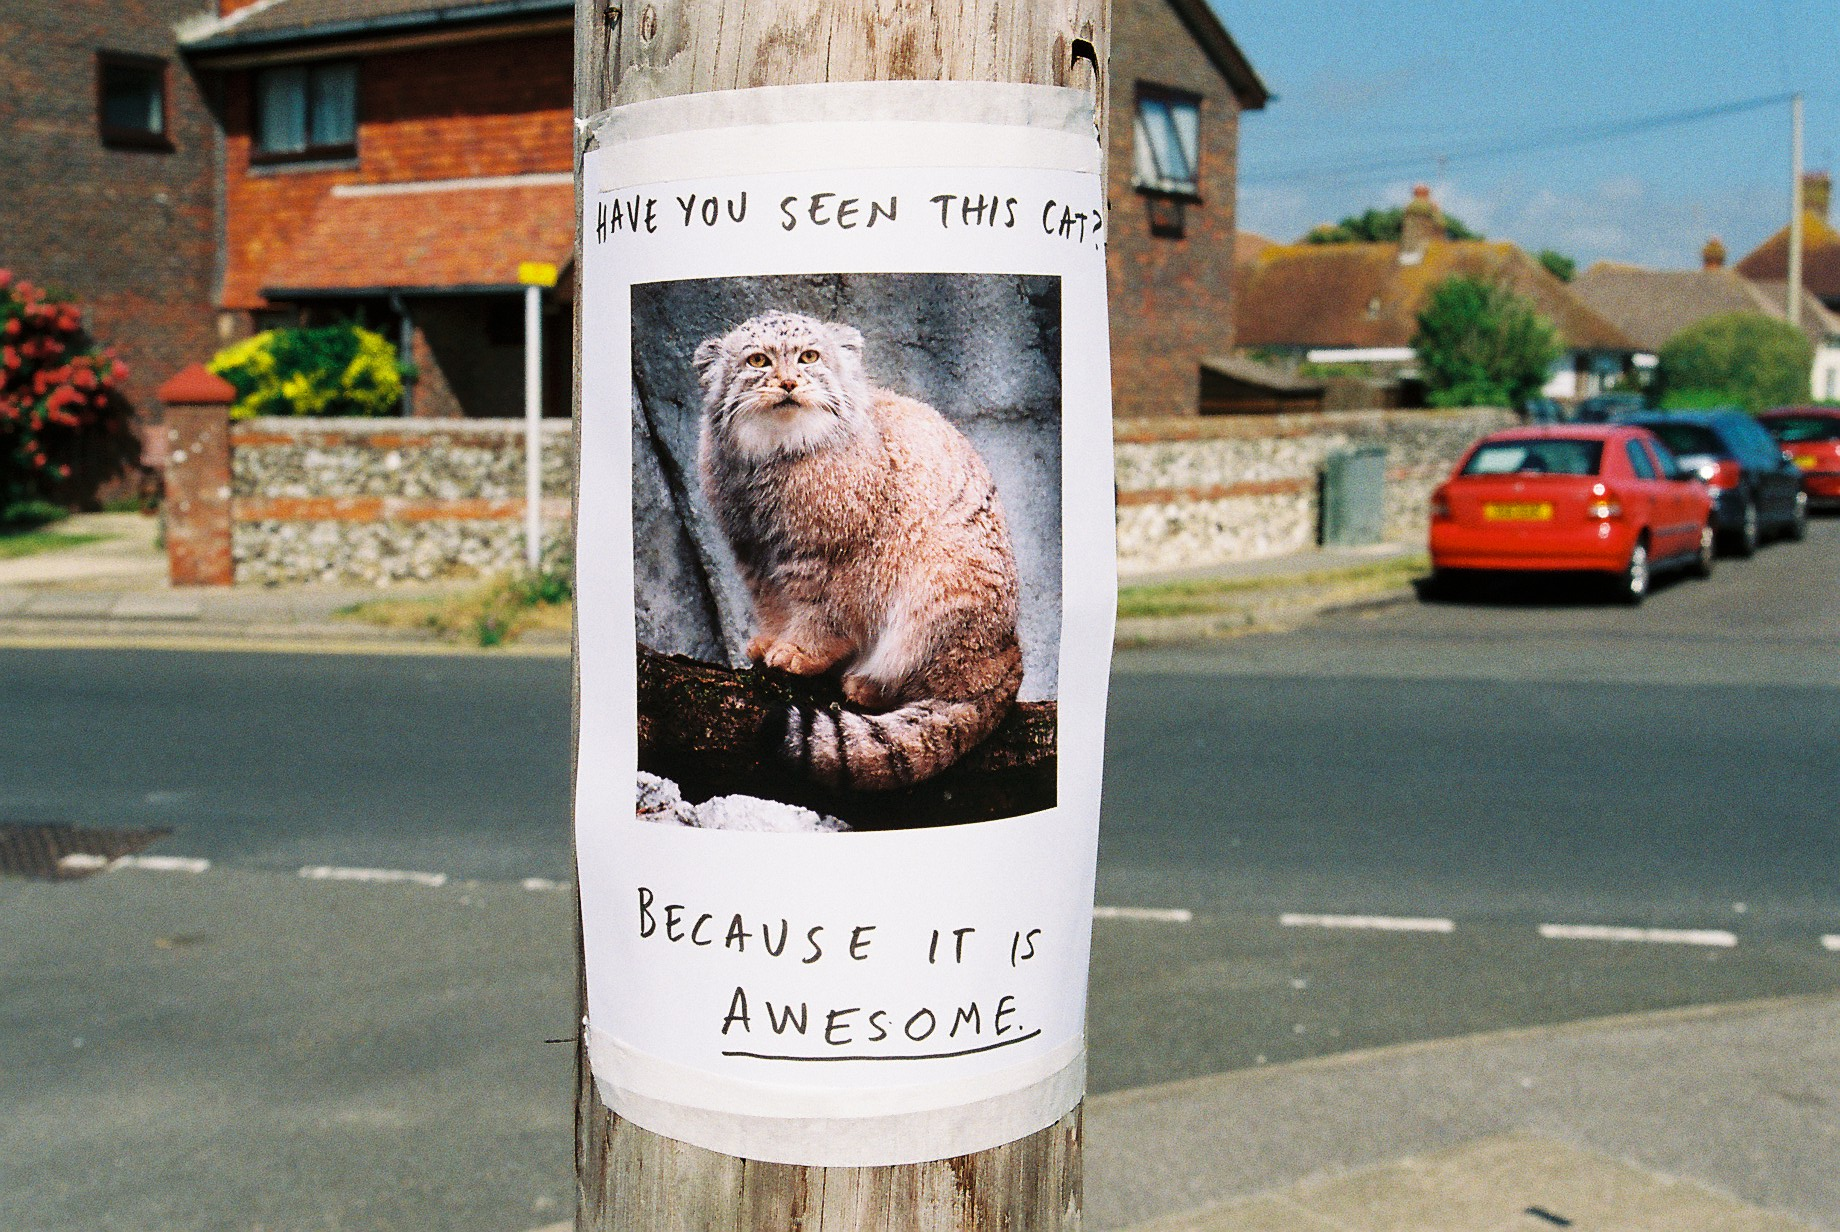
\includegraphics[width=0.5\textwidth]{./Figs/cat}
			\caption{Picture of an awesome cat.}
			\label{fig:awesomecat}
		\end{center}
	\end{figure}
	
	If you look at the \LaTeX\ code that generated this figure you will see that the figure width was set to $\frac{1}{2}$ the documents text width.
	Additionally a caption can be added to a figure using the \TT{\bs caption\{\tpc\}} command where the caption text is between the \TT{\{\tpc\}}.
	More information on figures can be found here: \url{https://en.wikibooks.org/wiki/LaTeX/Floats,_Figures_and_Captions}.
	
	\LaTeX\ also has the ability for you to draw your own pictures.
	We are not going to go into that for this presentation.
	But if you want to learn more about it, you can find out more here: \url{http://en.wikibooks.org/wiki/LaTeX/PGF/TikZ}
	
	\paragraph{Practice your figure and table skills by trying to replicate Exercise3.pdf}
	\clearpage
	
	%%%%%%%%%%%%%%%%%%%%%%%%%%%%
	%%%%% Space Management %%%%%
	%%%%%%%%%%%%%%%%%%%%%%%%%%%%
	
	\section{Space Management}
	\label{sec:spacemanagement}
	A great freedom (and curse) of \LaTeX\ is that you have free range to change mostly any spacing on the page.
	Sometimes you need to nudge something up, down, left, or right.
	The following section will discuss how to do this.
	
	\subsection{Units}
	\noindent Common units used in \LaTeX:
	\begin{itemize}
		\item pt - point (1 in = 72.27 pt)
		\item in - inch (1 in = 25.4 mm)
		\item cm - centimeter (1 cm = 10 mm)
		\item mm - millimeter
		\item em - roughly the width of an 'M' (uppercase) in the current font
		\item ex - roughly the height of an 'x' in the current font 
	\end{itemize}
	
	\noindent Useful \LaTeX\ measurements to reference:
	\begin{itemize}
		\item \TT{\bs textwidth} - The width of the text on the page (margin to margin)
		\item \TT{\bs textheight} - The height of the text on the page (margin to margin)
	\end{itemize}
	
	\subsection{Creating Whitespace}
	The following are commonly used commands for creating whitespace.
	
	\begin{itemize}
		\item \TT{\bs noindent} - Removes indent at the beginning of a new paragraph
		\item \TT{\bs} - About a single spacebar of spacing
		\item \TT{\bs quad} - About the spacing of `M'
		\item \TT{\bs qquad} - Add the spacing of `MM'
		\item \TT{\bs vspace\{\tpc\}} and \TT{vspace*\{\tpc\}} - Add vertical space of \TT{\{\tpc\}} units(*indicates manual override)
		\item \TT{\bs hspace\{\tpc\}} and \TT{hspace*\{\tpc\}} - Add horizontal space of \TT{\{\tpc\}} units (*indicates manual override)
		\item \TT{\bs vfill} - Adds whitespace to fill the page vertically
		\item \TT{\bs hfill} - Adds whitespace to fill the page horizontally
	\end{itemize}
	
	\subsection{Minipages}
	Sometimes you want to section out a page into subsections of space making it easier to manipulate sets of objects or place objects relative to one another.
	This can be difficult to do traditionally in \LaTeX\ but minipages can be used to make it easier.
	Minipages is somewhat analogous to axes in MATLAB.
	The general syntax for minpages is as follows:
	\begin{center}
		\TT{\bs begin\{minipage\}[pos][height][contentpos]\{width\}}\\
	\end{center}
	Minipages are a somewhat advanced feature and we will not go into too much detail on the topic here yet they are used quite a bit in the \TT{Slides\_Template.tex} file that will be shared with you after the workshop.
	
	\paragraph{Practice your whitespace management by trying to replicate Exercise4.pdf}
	\clearpage
	
	\section{Custom commands}
	\label{sec:customcommands}
	When using commands that can be tedious to type (e.g. \TT{\bs partial}), we can create new command handles that are easier to type out.
	For this one, we created a command such that \TT{\bs del} also gives us the same symbol as \TT{\bs partial}.
	At the beginning of the document, you can see where we typed this:
	\begin{center}
		\TT{\bs newcommand\{\bs del\}\{\bs partial\}} \\
	\end{center}
	So now we can retype Eqn. \eqref{eq:exampledel} using \TT{\bs del} instead of \TT{\bs partial} and we get the same result:
	\begin{align*}
		F(x) = \left\{ 
		\begin{array}{ll}
			0, & x \leq 0 \\
			\dfrac{\del u}{\del y} + C_1^2  & x > 0\\
		\end{array}
		\right. 
	\end{align*}
	\vspace{1cm}
	
	\begin{center}
		\textbf{Can you find the other custom commands that we made in this document?}
	\end{center}
	
	\clearpage
	\section{Bibliographies \& BibTeX}
	\label{sec:bibliography}
	As we have seen in the previous sections, \LaTeX\ is very very good at keeping track of the numbering of labels and compiling them in the proper order.
	This becomes EXTREMELY useful when it comes to creating a bibliography.
	In short, with the use of \hologo{BibTeX} a handle can be assigned to each reference.
	When you would like to cite the reference in writing all you need to do is use the command \TT{\bs cite\{\tpc\}}.
	\LaTeX\ will take care of the rest!
	
	\subsection{Using \hologo{BibTeX}}
	Creating bibliographies in \LaTeX\ is easy using \hologo{BibTeX}.
	\hologo{BibTeX} is awesome and a simple extension of \LaTeX\ \cite{MyRef0}.
	
	\begin{itemize}
		\item Information for references is stored in a separate \TT{.bib} file.
		\item For each reference the \TT{.bib} file will include an entry with your label for that reference and other relevant citation information such as author, title, journal, year, publisher, etc...
		\item These \TT{.bib} entries can usually be downloaded directly from the documents online source (eg., Google Scholar, Web of Knowledge, Elsevier, etc...) or generated with a third party literature management software such as Mendeley.
		\item Once the \TT{.bib} file is populated with reference entries and compiled, a reference can be cited in the text using \TT{\bs cite\{ReferenceLabel\}}.
		This will automatically add the reference to the bibliography and keep things in the order defined by the bibliography style being used.
		\item At the end of your document you will define the bibliography style using the command \TT{\bs bibliographystyle\{\tpc\}} and then point \LaTeX\ to your BibTex file name using the command \TT{\bs bibliography\{Filename.bib\}}
		\begin{itemize}
			\item There are many different bibliography styles and many journals will have their own style defined which you can just insert in your manuscript writing.
			Here we are using IEEE Transactions which is a standard built in style in \LaTeX.
		\end{itemize}
	\end{itemize}
	Take a look at the code that generated the citation at the beginning of this subsection and the corresponding \hologo{BibTeX} file to see how it was done.
	
	\subsection{Creating a \hologo{BibTeX} File and Entry Content}
	Creating a \TT{.bib} file is super easy.
	All you need to do is open a new file in \LaTeX, include the references, and save it as a \TT{.bib}.
	There is no limit to how many references you put in your \TT{.bib} file and only the ones that are cited will show up in the reference section.
	There is no need for a document class definition at the top of your \TT{.bib} file or any \TT{\bs begin\{\tpc\}} or \TT{\bs end\{\tpc\}} statements necessary.
	Like stated above, you can easily pull \hologo{BibTeX} citations from Google Scholar, but it is important to understand the content of a \hologo{BibTeX} entry.
	A sample reference entry for the \TT{.bib} file is shown below.
	\begin{verbatim}
	@article{hawking1982,
	title={The development of irregularities in a single bubble inflationary universe},
	author={Hawking, Stephen W},
	journal={Physics Letters B},
	volume={115},
	number={4},
	pages={295--297},
	year={1982},
	publisher={Elsevier}
	}
	\end{verbatim}
	More information on different types of entries can be found here: \url{https://en.wikipedia.org/wiki/BibTeX}
	
	\paragraph{Practice your \hologo{BibTeX} skills by trying to replicate Exercise5.pdf}
	
	\clearpage
	\section{Other Random Resources}
	\begin{itemize}
		\item Templates - Can pull pre-generated style and class files for a specific document type (\url{http://www.latextemplates.com/})
		\item Mathematica - Can copy inputs and outputs as \LaTeX\, great for large tables and matrices
		\item Detexify - Can draw symbols and it will output the \LaTeX\ command (\url{http://detexify.kirelabs.org/classify.html})
		\item Codecogs  - Real time typing of \LaTeX\ math equations with a helpful user interface (\url{https://www.codecogs.com/latex/eqneditor.php})
	\end{itemize}
	
	\clearpage
	\bibliographystyle{ieeetr}
	\bibliography{MyBib}
\end{document}

